\documentclass[11pt,a4paper]{article}

% --- Packages ---
\usepackage[utf8]{inputenc}
\usepackage[T1]{fontenc}
\usepackage{amsmath,amssymb,amsthm}
\usepackage{mathtools}
\usepackage{booktabs}
\usepackage{graphicx}
\usepackage[colorlinks=true,citecolor=blue,linkcolor=blue,urlcolor=blue]{hyperref}
\usepackage{geometry}
\usepackage{setspace}
\usepackage[expansion=false,protrusion=false]{microtype}
\usepackage{tikz}
\usetikzlibrary{shapes,arrows,positioning,fit,calc}
\usepackage{xcolor}

\definecolor{codeblue}{RGB}{0,102,204}
\definecolor{darkgreen}{RGB}{0,128,0}

\newtheorem{theorem}{Theorem}[section]
\newtheorem{definition}{Definition}[section]
\newtheorem{proposition}{Proposition}[section]
\newtheorem{lemma}{Lemma}[section]
\newtheorem{corollary}{Corollary}[section]

% --- Page geometry ---
\geometry{
  top=1in,
  bottom=1in,
  left=1.1in,
  right=1.1in,
}

\setstretch{1.08}

% --- Title ---
\title{
  \vspace{-1.5cm}
  \textbf{Synchra: A Privacy-Preserving Programmable Leverage\\[4pt]
  and Yield Layer for Arc}
  \vspace{-0.3cm}
}

\author{
  Synchra Protocol Contributors\\[4pt]
  \texttt{https://synchra.org}
}

\date{}

\begin{document}

\maketitle
\thispagestyle{empty}

\vspace{0.3cm}

\begin{abstract}
  \noindent Circle's Arc blockchain provides institutional-grade settlement infrastructure -- deterministic sub-second finality, USDC-native gas, and EVM compatibility -- and is explicitly designed as a foundational layer for stablecoin finance, programmable FX, tokenized assets, and agent-driven treasury operations. What Arc does not yet provide is a shared market infrastructure that turns settlement into capital-efficient markets: a unified clearing kernel where USDC, EURC, and yield-bearing collateral such as USYC can back FX hedges, tokenized-asset positions, leveraged strategies, and autonomous agent portfolios under a single portfolio risk framework.

  We present \textbf{Synchra}, a privacy-preserving, programmable leverage and yield layer purpose-built for Arc. Synchra is differentiated by three defensible moats: \textbf{(i) leverage} -- portfolio-level margin, collateral reuse across heterogeneous markets, and internal repo/rehypothecation; \textbf{(ii) privacy} -- encrypted order flow, RFQs, batch auctions, TEE-based matching, and forward compatibility with Arc's protocol-level privacy roadmap (APS); and \textbf{(iii) programmable yield} -- USYC-bearing collateral tiers, autonomous strategy vaults, and agent-controlled smart treasuries. The protocol supports perpetual swaps, FX derivatives, real-world asset markets, programmable strategy vaults, and yield-bearing collateral pools within one unified risk and settlement system.

  Synchra integrates directly with Circle's platform -- USDC/EURC settlement, USYC yield-bearing collateral, CCTP cross-chain liquidity, Circle's Agent Stack, Nanopayments, and Developer Controlled Wallets -- and is designed to remain composable with Arc's native privacy roadmap. This paper presents the architecture, formalizes the clearing kernel and portfolio margin model, and analyzes security and economic properties.
\end{abstract}

\vspace{0.3cm}

\noindent\textbf{Keywords:} decentralized finance, portfolio margin, leverage, privacy-preserving execution, yield-bearing collateral, programmable vaults, onchain settlement

\newpage
\tableofcontents
\newpage

%=============================================================================
\section{Introduction}
\label{sec:introduction}
%=============================================================================

Circle's Arc blockchain~\cite{circlearc} delivers what blockchains were always meant to be: a settlement layer for programmable money with institutional-grade performance. Combining Malachite consensus with EVM compatibility, Arc achieves deterministic sub-second finality, low-latency throughput, and USDC as native gas~\cite{arc_technical}. Circle describes Arc as the Economic OS for the internet -- a stablecoin-native Layer-1 optimized for global payments, programmable FX, tokenized assets, and agent-driven financial workflows.

Yet a settlement chain is not a market. While Arc provides the rails for value movement, it does not yet provide the shared clearing, risk, and execution infrastructure that would allow diverse financial applications to share capital and settle against one another. A lending protocol, an FX hedging venue, and a tokenized-asset derivatives market launching on Arc would each rebuild its own collateral pool, risk engine, and settlement logic. The result is fragmented capital, duplicated fixed costs, and a market layer that develops more slowly than the underlying chain.

The core opportunity is therefore architectural. Modern finance runs on shared clearing infrastructure: central counterparties, prime brokers, and tri-party settlement systems allow collateral to flow across desks, markets, and jurisdictions. In decentralized finance, smart contracts have historically collapsed execution, clearing, and settlement into monolithic applications. This worked for simple token swaps, but it fails for the diverse, interconnected markets that define institutional finance.

\textbf{Synchra} introduces a privacy-preserving, programmable leverage and yield layer for Arc. It separates execution from clearing and settlement, enabling any market primitive to plug into a unified collateral pool and risk engine. Synchra's competitive position rests on three mutually reinforcing moats:

\begin{enumerate}
  \item \textbf{Leverage through portfolio-level margin.} Synchra computes margin across all of a user's positions, across all market types. A long EURC/USDC FX hedge can offset a USDC-denominated perpetual position; cross-chain collateral via CCTP increases effective capital without forcing pre-positioning; and an internal repo/securities-lending module enables collateral reuse within a unified risk framework. Leverage here is not merely high multiplier exposure -- it is the systematic reuse and optimization of collateral, which increases returns on deposited capital and deepens liquidity for every market plugged into the kernel.

  \item \textbf{Privacy through encrypted execution.} Institutional participants will not move size onchain if their order flow, positions, and strategies are visible to the mempool or to block proposers. Synchra provides configurable privacy -- public CLOBs for transparent markets, encrypted RFQs for block trades, TEE-based matching for confidential order flow, and zero-knowledge solvency attestations -- all operating as an application-layer complement to Arc's protocol-level privacy roadmap.

  \item \textbf{Programmable yield on productive collateral.} A clearing layer that merely holds collateral is capital inefficient. Synchra treats idle margin as productive capital: USYC and other yield-bearing assets earn yield while simultaneously backing positions, and programmable strategy vaults deploy collateral into delta-neutral, FX carry, funding-arbitrage, and RWA-backed strategies -- all margined through the same kernel.
\end{enumerate}

The result is that Synchra turns Arc from a settlement chain into a capital-efficient market infrastructure. Traders, enterprises, asset managers, and autonomous agents can run multi-strategy, multi-currency, cross-market portfolios from a single collateral pool, with deterministic settlement finality and fees denominated in USDC.

\subsection{Thesis}

We argue that Arc's full potential as a financial settlement layer requires a shared clearing, risk, and yield infrastructure that is currently missing. Synchra provides this infrastructure. Rather than launching another monolithic exchange, Synchra separates execution from clearing and settlement, enabling any market primitive to plug into a unified collateral pool, portfolio risk engine, and yield framework. The result is not a single protocol but a platform: a privacy-preserving, capital-efficient leverage and yield layer for stablecoin-native markets on Arc.

Synchra realizes this through:

\begin{itemize}
  \item \textbf{A unified clearing kernel} providing shared accounting, collateral management, settlement, and portfolio-level risk assessment across all markets on Arc.
  \item \textbf{A modular market extension framework} allowing financial primitives -- FX derivatives, perpetuals, RWA markets, strategy vaults -- to be deployed as kernel extensions without replicating infrastructure.
  \item \textbf{A portfolio margin engine} evaluating correlated positions across heterogeneous markets, enabling collateral reuse and systematic hedging credits impossible under isolated margin.
  \item \textbf{Configurable privacy} through encrypted order flow, RFQs, batch auctions, and TEE-based matching -- an application-layer privacy layer that is composable with Arc's protocol-level privacy roadmap (APS).
  \item \textbf{Programmable yield infrastructure} including USYC-bearing collateral tiers, strategy vaults, internal repo markets, and agent-controlled smart treasuries.
  \item \textbf{Agent-native participation} with programmable agent accounts, session policies, and direct integration with Circle's agent and payment infrastructure.
  \item \textbf{Stablecoin-native settlement} via USDC and EURC, with USYC and other yield-bearing assets as collateral, and CCTP for cross-chain liquidity.
\end{itemize}

\subsection{Paper organization}

Section~\ref{sec:background} motivates the design through analysis of existing systems and the Arc ecosystem gap. Section~\ref{sec:model} formalizes the system model, actors, and design goals. Section~\ref{sec:architecture} presents the layered architecture. Sections~\ref{sec:clearing} through~\ref{sec:privacy} detail the clearing kernel, portfolio margin, programmable markets, execution layer, and privacy architecture. Sections~\ref{sec:agents},~\ref{sec:yield}, and~\ref{sec:economics} discuss agent-native markets, yield and strategy vaults, and economic security. Section~\ref{sec:arc} establishes how Synchra integrates with and complements the Arc ecosystem. Section~\ref{sec:related} surveys related work, and Section~\ref{sec:roadmap} outlines the implementation roadmap.

%=============================================================================
\section{Background and Motivation}
\label{sec:background}
%=============================================================================

\subsection{The Arc ecosystem gap}

Arc delivers the technical foundation for institutional onchain finance: Malachite consensus for deterministic sub-second finality, a Reth-based EVM for full EVM compatibility, USDC as native gas for stable-denominated fees, and native integration with Circle's broader platform including USDC, EURC, CCTP, and USYC~\cite{circlearc, arc_technical}. Circle's broader platform adds tokenized money-market instruments (USYC), Nanopayments for gas-free microtransfers, the Agent Stack for autonomous financial agents, and CCTP bridging across chains.

Arc's public messaging explicitly targets stablecoin-native use cases: global payments, programmable FX, tokenized assets, and agent-driven treasury operations~\cite{circlearc}. The ecosystem requires high-quality tokenized RWAs composable with DeFi primitives, institutional-grade FX infrastructure, and smart treasury agents. What is not on Arc's public roadmap is the shared clearing, risk, and yield layer that would allow these applications to share collateral and settle against one another. That is Synchra's opportunity.

\subsection{Evolution of decentralized markets}

DeFi derivatives have progressed through several architectural generations:

\textbf{First generation} (2020--2021) established AMM-based perpetuals. These used virtual AMMs for price discovery, inheriting liquidity limitations from spot AMMs.

\textbf{Second generation} (2021--2023) introduced hybrid models. Liquidity-pool protocols used pooled collateral as counterparty, enabling deep markets without orderbooks but exposing liquidity providers to concentrated and often asymmetric risk.

\textbf{Third generation} (2023--2025) brought orderbook-based derivatives to dedicated execution environments. These environments demonstrated that onchain CLOBs could match centralized exchange latency, and several protocols began introducing portfolio margin concepts within single asset classes.

\textbf{Concurrent innovations} include modular exchange extensibility, private execution via zero-knowledge and TEE-based matching, the emergence of tokenized money-market funds as yield-bearing collateral, and clearing-focused architectures that separate clearing, margin, and execution layers.

\subsection{Lessons from clearing-focused architectures}

Modern clearing-focused exchange architectures validate several principles that Synchra adopts:

\begin{itemize}
  \item \textbf{Layer separation.} Clearing, risk, and execution should be independent components with clean interfaces.
  \item \textbf{Account-level cross margin.} Margin requirements should be computed at the account level rather than per-position.
  \item \textbf{Multi-tier liquidation cascade.} Standard liquidation, backstop liquidation, and auto-deleveraging provide a robust default waterfall.
  \item \textbf{Per-second funding accrual.} Cadence-invariant funding simplifies position accounting.
\end{itemize}

Synchra applies these principles specifically for Arc. Arc's deterministic sub-second finality removes the need for custom consensus clusters or geographic colocation. Synchra's moats are leverage through cross-market portfolio margin, privacy through encrypted execution, and programmable yield through yield-bearing collateral and strategy vaults. Synchra is designed for the stablecoin-native, agent-driven market layer Arc is building toward.

\subsection{Architectural principles}

Our design is shaped by several hard-won lessons from the evolution of on-chain trading infrastructure:

\begin{enumerate}
  \item \textbf{Separate concerns.} Clearing, risk, and execution should be independent systems with narrow interfaces. This allows each layer to be optimized, scaled, and audited independently, and makes the protocol robust to changes in any one layer.

  \item \textbf{Shard by account and market.} Most financial operations touch only two parties and one market. Designing state around accounts and markets enables parallel execution and horizontal scaling without global coordination.

  \item \textbf{On-chain settlement truth, off-chain latency.} Final collateral balances, positions, and obligations must be verifiable on-chain. Off-chain components should only handle sequencing, privacy, or computation that can be independently verified.

  \item \textbf{Gas-aware market design.} Gas cost is a market-structure variable, not an implementation detail. Hot paths such as post, cancel, and modify must be storage-efficient so that market makers can quote tight spreads.

  \item \textbf{Cadence-invariant economics.} Funding, yield, and fee accrual should be continuous functions of time and state, so that a participant's PnL does not depend on when a settlement event happens.

  \item \textbf{Staged default waterfall.} Insolvency should escalate through a predictable ladder: standard liquidation, backstop liquidation, auto-deleveraging, and finally contract unwind. Clarity prevents panic-driven cascades.

  \item \textbf{Oracle-tethered mark pricing.} A derivative's mark price should be anchored tightly to the underlying spot price through multiple independent feeds, with impact-based pricing to resist manipulation.

  \item \textbf{Permissionless safety functions.} Liquidation, funding settlement, and proof verification should not require privileged operators. Anyone must be able to enforce protocol solvency.

  \item \textbf{Economic cleanup incentives.} Markets produce garbage: expired orders, stale quotes, dust positions. The protocol should pay participants to remove them.

  \item \textbf{Compartmentalized risk with global backstops.} Risk should be isolated by market and vault so that one failure does not contaminate the whole system, but a global backstop should exist for tail events.

  \item \textbf{Colocate with the economic center.} Execution infrastructure should sit as close as possible to the source of economic activity. For Synchra on Arc, this means native integration with USDC, EURC, USYC, CCTP, Circle's Agent Stack, and Nanopayments -- not treating Arc as one of many supported chains.
\end{enumerate}

\subsection{Limitations of current architectures}

Despite these advances, all existing systems share fundamental constraints:

\textbf{Exchange-centric architecture.} Every protocol is built as a standalone exchange. This requires each to bootstrap liquidity, develop a risk engine, and manage settlement independently. The economics of marginal benefit and high fixed cost create natural monopolies.

\textbf{Single-market risk.} Margin is computed per-position or per-market. A trader with offsetting positions across protocols receives no cross-margin benefit. Even within protocols supporting multiple markets, risk aggregation is typically additive rather than portfolio-based.

\textbf{Transparency as default.} Onchain execution reveals order parameters -- price, size, side, leverage -- to the mempool or block proposer before execution. This enables MEV extraction estimated at hundreds of millions annually~\cite{mev} and deters institutional flow.

\textbf{Closed extension models.} Adding a new market type requires forking and redeploying. There is no standard interface for plugging new financial primitives into existing risk and clearing infrastructure.

\textbf{Capital isolation.} Collateral deposited in one protocol is inaccessible to others, even when the same asset is used. This fragments what should be a single pool of systemic collateral.

\subsection{Research contribution}

Synchra's contribution is an architectural synthesis that advances the state of onchain financial infrastructure while aligning closely with Arc's stated priorities. The specific contributions are:

\begin{enumerate}
  \item \textbf{A clearing kernel for Arc.} Synchra provides a shared clearing, risk, and collateral infrastructure for capital markets on Arc -- deployed as modular extensions rather than isolated protocols.
  \item \textbf{Clearing kernel formalization.} We define a minimal interface for onchain clearing that separates market logic from risk, collateral, and settlement, and argue that any market satisfying the kernel interface can share a unified collateral pool without compromising kernel invariants. A full invariant proof is left to a companion specification document accompanying the reference implementation.
  \item \textbf{Portfolio margin across heterogeneous markets.} We extend portfolio-based margin (present in traditional futures clearing houses and in some single-asset-class onchain protocols) to a heterogeneous market model supporting perpetuals, FX derivatives, RWA markets, and strategy vaults simultaneously within one collateral pool.
  \item \textbf{Privacy-preserving execution.} We design a configurable privacy architecture that spans encrypted order flow, RFQs, batch auctions, TEE-based matching, and ZK solvency attestation, without requiring full ZK matching for every order.
  \item \textbf{Programmable yield framework.} We integrate yield-bearing collateral tiers, internal repo, and strategy vaults into the clearing kernel so that collateral can earn yield while backing positions.
  \item \textbf{Agent-native design.} We specify autonomous agents as first-class clearing participants with programmable permissions, session keys, and direct integration with Circle's Agent Stack and Nanopayments.
\end{enumerate}

%=============================================================================
\section{System Model}
\label{sec:model}
%=============================================================================

\subsection{Actors}

Synchra defines five participant types:

\begin{description}
  \item[Traders] Human or automated participants who open, modify, and close positions. Traders interact through the execution layer and maintain accounts in the clearing kernel.
  \item[Institutions] Organizations with multi-user access control, compliance requirements, and portfolio-level risk management. Institutions have hierarchical account structures with sub-account isolation.
  \item[Agents] Autonomous programs registered as protocol participants with cryptographic identities, programmable permissions, and execution policies. Agents are first-class accounts, not scripts operated by traders.
  \item[Liquidity providers] Participants who deposit collateral into liquidity pools for specific markets, earning fees and funding payments in exchange for assuming inventory risk.
  \item[Validators/Sequencers] Infrastructure operators responsible for transaction ordering, state transitions, and in the case of TEE execution, attestation of confidential computations.
\end{description}

\subsection{Threat model}

Synchra assumes the following threat landscape:

\begin{itemize}
  \item \textbf{Consensus layer security} is provided by the underlying chain (Arc EVM). We assume consensus is Byzantine fault tolerant.
  \item \textbf{Smart contract risk} is managed through formal verification of the clearing kernel and independent audits of market extensions.
  \item \textbf{Oracle manipulation} is mitigated through redundant oracle feeds, TWAP-based pricing, and circuit breakers.
  \item \textbf{MEV and front-running} are addressed through encrypted order flow, batch auctions, and fair ordering within the execution layer.
  \item \textbf{TEE trust} requires trust in hardware manufacturers (Intel TDX/AMD SEV-SNP). We treat TEE compromise as low-probability but provide ZK fallback for verification.
  \item \textbf{Privacy leakage} through side channels (metadata, timing, network analysis) is acknowledged as a limitation of the current architecture.
\end{itemize}

\subsection{Design goals}

\begin{description}
  \item[G1 --- Unified liquidity.] Collateral deposited in the clearing kernel must be available to support positions in any market extension, subject to portfolio-level risk constraints.
  \item[G2 --- Portfolio risk.] Margin requirements must be computed holistically across all of a trader's positions, incorporating correlation, hedging, concentration, and liquidity factors.
  \item[G3 --- Modular markets.] Any financial primitive satisfying the kernel's market extension interface must be deployable without modifying the core clearing logic.
  \item[G4 --- Leverage and capital efficiency.] The system must maximize collateral reuse -- yield-bearing collateral, cross-market hedging credits, and cross-chain collateral -- while controlling default risk.
  \item[G5 --- Configurable privacy.] Users must control the confidentiality level of each order and position, from fully public to encrypted/TEE-protected execution with selective disclosure.
  \item[G6 --- Agent compatibility.] Autonomous agents must be native protocol participants with programmable permissions, cryptographic identities, and execution policies.
  \item[G7 --- Deterministic settlement.] Settlement must be deterministic and independently verifiable from execution, ensuring that the clearing kernel remains the authoritative source of financial truth.
  \item[G8 --- Yield-bearing collateral.] Collateral must generate yield while backing positions, so that capital efficiency includes passive income as well as leverage.
\end{description}

%=============================================================================
\section{Synchra Architecture}
\label{sec:architecture}
%=============================================================================

Synchra is organized as a layered architecture, where each layer abstracts a distinct concern and communicates through well-defined interfaces.

\begin{figure}[h]
  \centering
  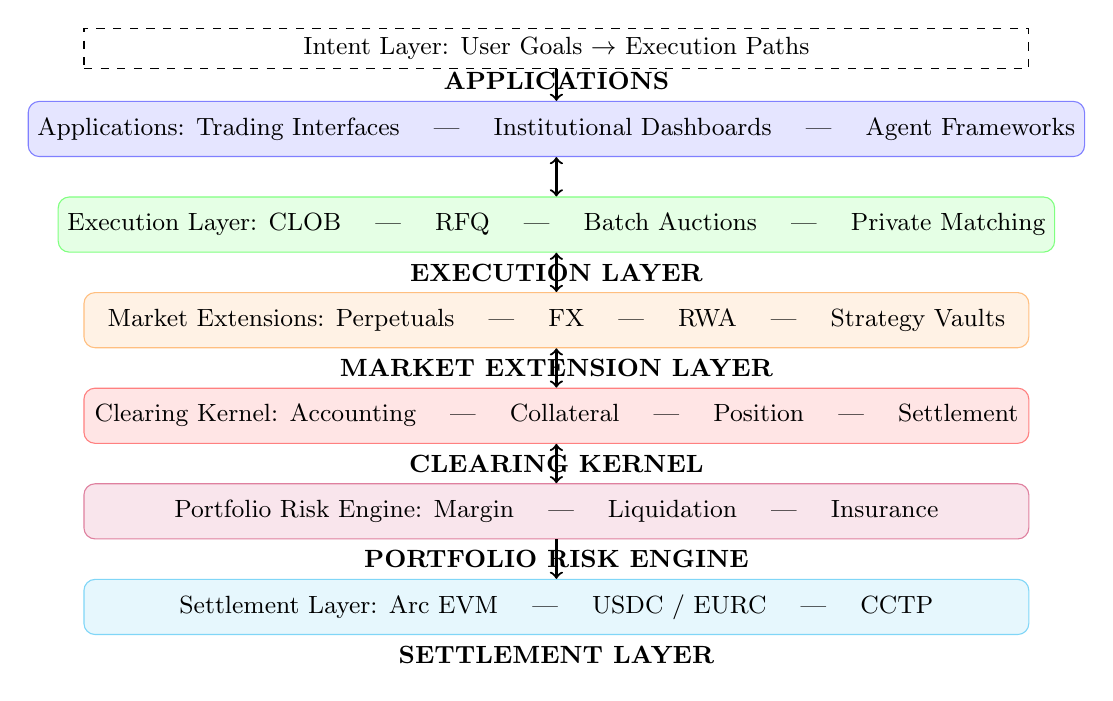
\begin{tikzpicture}[
    layer/.style={rectangle, draw, rounded corners, minimum width=12cm, minimum height=0.7cm, font=\small},
    app/.style={layer, fill=blue!10, draw=blue!50},
    exec/.style={layer, fill=green!10, draw=green!50},
    mkt/.style={layer, fill=orange!10, draw=orange!50},
    clear/.style={layer, fill=red!10, draw=red!50},
    risk/.style={layer, fill=purple!10, draw=purple!50},
    settle/.style={layer, fill=cyan!10, draw=cyan!50},
    label/.style={font=\small\bfseries, align=center}
  ]
    % Applications
    \node[app] (apps) {Applications: Trading Interfaces \quad | \quad Institutional Dashboards \quad | \quad Agent Frameworks};
    \node[label, above=0.02cm of apps] {APPLICATIONS};

    % Intent Layer
    \node[draw, dashed, minimum width=12cm, minimum height=0.5cm, font=\small, above=0.4cm of apps] (intent) {Intent Layer: User Goals $\rightarrow$ Execution Paths};

    % Execution Layer
    \node[exec, below=0.5cm of apps] (execution) {Execution Layer: CLOB \quad | \quad RFQ \quad | \quad Batch Auctions \quad | \quad Private Matching};
    \node[label, below=0.02cm of execution] {EXECUTION LAYER};

    % Market Extensions
    \node[mkt, below=0.5cm of execution] (markets) {Market Extensions: Perpetuals \quad | \quad FX \quad | \quad RWA \quad | \quad Strategy Vaults};
    \node[label, below=0.02cm of markets] {MARKET EXTENSION LAYER};

    % Clearing Kernel
    \node[clear, below=0.5cm of markets] (clearing) {Clearing Kernel: Accounting \quad | \quad Collateral \quad | \quad Position \quad | \quad Settlement};
    \node[label, below=0.02cm of clearing] {CLEARING KERNEL};

    % Portfolio Risk Engine
    \node[risk, below=0.5cm of clearing] (risk) {Portfolio Risk Engine: Margin \quad | \quad Liquidation \quad | \quad Insurance};
    \node[label, below=0.02cm of risk] {PORTFOLIO RISK ENGINE};

    % Settlement
    \node[settle, below=0.5cm of risk] (settlement) {Settlement Layer: Arc EVM \quad | \quad USDC / EURC \quad | \quad CCTP};
    \node[label, below=0.02cm of settlement] {SETTLEMENT LAYER};

    % Arrows
    \draw[->, thick] (intent.south) -- (apps.north);
    \draw[<->, thick] (apps.south) -- (execution.north);
    \draw[<->, thick] (execution.south) -- (markets.north);
    \draw[<->, thick] (markets.south) -- (clearing.north);
    \draw[<->, thick] (clearing.south) -- (risk.north);
    \draw[->, thick] (risk.south) -- (settlement.north);
  \end{tikzpicture}
  \caption{Synchra layered architecture. Arrows indicate bidirectional communication except between the risk engine and settlement layer, where settlement is downstream.}
  \label{fig:architecture}
\end{figure}

\subsection{Architectural philosophy}

The architecture follows three principles:

\begin{enumerate}
  \item \textbf{Separation of concerns.} Each layer is independently upgradeable and testable. Market extensions cannot compromise the clearing kernel's invariants.

  \item \textbf{Minimal core, maximal extension.} The clearing kernel implements only what is universally required: accounting, collateral management, and settlement. Market-specific logic lives in extensions.

  \item \textbf{Deterministic settlement.} The clearing kernel's state transitions are deterministic functions of authenticated market outputs. Execution may involve off-chain computation (matching, risk evaluation), but settlement always reduces to onchain state transitions.
\end{enumerate}

\subsection{Layer responsibilities}

\textbf{Application layer.} Frontends, dashboards, and agent frameworks that translate user intent into protocol actions. The application layer communicates through the intent layer, which abstracts execution path selection.

\textbf{Execution layer.} Handles order matching, price discovery, and trade execution. Supports multiple execution modes: a public CLOB for transparent markets, an RFQ system for block trades, batch auctions for fairness, and a private matching engine for confidential orders.

\textbf{Market extension layer.} Contains the financial logic for specific market types. Each extension implements the `IMarket` interface defined by the clearing kernel and manages market-specific state: funding rates, leverage parameters, oracle feeds, and resolution mechanisms.

\textbf{Clearing kernel.} The core financial state machine: account abstraction, collateral vault, position tracking, and settlement engine. The kernel is market-agnostic -- it manages balances and positions without understanding their semantics.

\textbf{Portfolio risk engine.} Computes collateral requirements across all of a trader's positions. Runs liquidations when requirements are breached. Manages the insurance fund. The risk engine is the only component with a global view of trader positions.

\textbf{Settlement layer.} The underlying chain infrastructure. Synchra is designed for Arc EVM, leveraging native USDC/EURC settlement, CCTP for cross-chain transfers, and Arc's low-latency finality.

Each layer communicates through a narrow interface. The execution layer does not hold collateral; the risk engine does not match orders; the clearing kernel does not price markets. This separation is the foundation of Synchra's modularity and security.

%=============================================================================
\section{Clearing Kernel}
\label{sec:clearing}
%=============================================================================

The clearing kernel is the central state machine of Synchra. It maintains the authoritative record of accounts, collateral, positions, and obligations. All market extensions settle through the kernel, ensuring that settlement is unified even when execution is distributed.

The kernel is intentionally minimal. It does not understand market semantics; it understands debits, credits, and the interface through which extensions request changes to account state. This minimalism keeps the trusted computing base small and makes formal verification tractable.

\subsection{Account model}

Each participant has a \textbf{clearing account} that aggregates:
\begin{itemize}
  \item \textbf{Collateral balance} by asset type (USDC, EURC, USYC, and accepted tokenized assets).
  \item \textbf{Position set} across all market extensions, keyed by market ID.
  \item \textbf{Credit record} for funding payments, fees, and liquidation penalties.
\end{itemize}

Formally, an account $A$ is a tuple:
\[
A = (\mathcal{B}, \mathcal{P}, \mathcal{H})
\]
where $\mathcal{B}$ is a vector of collateral balances $\{b_a \mid a \in \mathcal{A}\}$, $\mathcal{P}$ is a set of positions $\{p_m \mid m \in \mathcal{M}\}$ indexed by market, and $\mathcal{H}$ is a credit/debit history.

\subsection{Collateral engine}

The collateral engine manages deposits, withdrawals, and valuations. Assets are classified by their \textbf{collateral tier}, determining haircuts and eligibility. This four-tier classification (Table~\ref{tab:collateral}) is the single authoritative tier taxonomy used throughout this paper; Section~\ref{sec:yield} describes how each tier accrues yield, and treats cross-chain origin as a haircut modifier applied on top of a tier rather than a tier of its own.

\begin{table}[h]
  \centering
  \begin{tabular}{lll}
    \toprule
    \textbf{Tier} & \textbf{Assets} & \textbf{Haircut} \\
    \midrule
    1 & USDC, EURC & 0\% \\
    2 & USYC, stUSD & 2\%--5\% \\
    3 & ETH, BTC (liquid staking) & 10\%--20\% \\
    4 & Tokenized RWAs & 15\%--35\% \\
    \bottomrule
  \end{tabular}
  \caption{Collateral tiers and haircuts. Haircuts are dynamic and adjusted by the risk engine based on volatility and liquidity conditions. An additional cross-chain modifier (typically +2\%--5\% haircut) applies to any tier-eligible asset bridged via CCTP rather than natively held on Arc, reflecting bridging and rebalancing latency.}
  \label{tab:collateral}
\end{table}

The effective collateral value for an account is:
\[
\mathcal{C}_{\text{eff}} = \sum_{a \in \mathcal{A}} b_a \cdot (1 - h_a) \cdot p_a
\]
where $b_a$ is the balance, $h_a$ the haircut (inclusive of any cross-chain modifier), and $p_a$ the oracle price of asset $a$.

\subsection{Position engine}

The position engine maintains the position set $\mathcal{P}$ for each account. A position $p_m$ in market $m$ is defined by extension-specific data but must expose a canonical interface:

\begin{figure}[h]
  \caption{IMarket interface (simplified)}
  \label{alg:market}
  \begin{quote}
  \texttt{\textbf{struct} MarketPosition:} \\
  \texttt{\qquad marketId: bytes32} \\
  \texttt{\qquad size: int256 \hfill // Positive = long, negative = short} \\
  \texttt{\qquad entryPrice: uint256} \\
  \texttt{\qquad margin: uint256} \\
  \texttt{\qquad leverage: uint256 \hfill // Per-market risk-tier ceiling, not effective leverage} \\
  \texttt{\textbf{function} getPnL(oraclePrice) $\rightarrow$ int256} \\
  \texttt{\textbf{function} getFunding(position, period) $\rightarrow$ int256} \\
  \texttt{\textbf{function} validateOpen(size, collateral) $\rightarrow$ bool} \\
  \texttt{\textbf{function} validateClose(position) $\rightarrow$ bool}
  \end{quote}
\end{figure}

The kernel stores positions as opaque bytes with typed accessors, allowing the kernel to remain market-agnostic while the risk engine reads the data it needs.

The \texttt{leverage} field on \texttt{MarketPosition} denotes the maximum leverage \emph{ceiling} permitted for that position under its market extension's risk-tier configuration -- it is a per-market bound, not the trader's effective leverage. Because Synchra margins at the portfolio level (Section~\ref{sec:margin}), effective leverage is an emergent, account-level quantity computed by the portfolio risk engine as total notional exposure divided by effective collateral $\mathcal{C}_{\text{eff}}$, and cannot be read off a single position.

\subsection{Settlement engine}

The settlement engine processes three types of events:

\textbf{Trade settlement.} When a match occurs in the execution layer, the settlement engine validates the matched trade against the risk engine, updates positions, and applies collateral changes atomically. Margin-based instruments (perpetuals, FX derivatives) require both counterparties to post initial margin against their new positions. Instruments that carry an upfront premium transfer the premium from buyer to seller at settlement.

\textbf{Funding settlement.} Funding accrues continuously from a per-market funding index. The settlement engine does not write every position's funding PnL to storage at every interval; instead, it updates the global funding index and computes a position's funding PnL lazily when the position changes. This cadence-invariant design ensures that funding payments are independent of the exact block at which settlement is triggered.

\textbf{Liquidation settlement.} When the risk engine flags an account, the settlement engine freezes the account's positions and delegates liquidation to the appropriate mechanism based on the default waterfall (Section~\ref{sec:margin}).

%=============================================================================
\section{Portfolio Margin Engine}
\label{sec:margin}
%=============================================================================

The portfolio margin engine is a principal differentiator of Synchra. Rather than margining each position independently, the engine evaluates the entire portfolio to determine capital requirements.

\subsection{Motivation}

In existing DeFi derivatives, a trader who is:
\begin{itemize}
  \item Long 10 BTC notional on Exchange A
  \item Short 9.5 BTC notional on Exchange B
\end{itemize}
posts margin on both positions, despite the net exposure being only 0.5 BTC. The gross margin requirement is approximately $(10 + 9.5) \times \text{IM}_\text{BTC} = 19.5 \times \text{IM}_\text{BTC}$, when the true economic requirement is $0.5 \times \text{IM}_\text{BTC}$.

Portfolio margin solves this by computing net risk at the account level.

\subsection{Margin model}

We define the portfolio margin requirement $\mathcal{M}(\mathcal{P})$ as a function of the position set $\mathcal{P}$:

\[
\mathcal{M}(\mathcal{P}) = f_S(\mathcal{P}) + f_C(\mathcal{P}) + f_L(\mathcal{P}) + f_K(\mathcal{P})
\]

Where:
\begin{itemize}
  \item $f_S(\mathcal{P})$ is the \textbf{scenario-based margin} component, computed as the maximum loss across a set of price scenarios $\mathcal{S}$:
  \[
  f_S(\mathcal{P}) = \max_{s \in \mathcal{S}} \left( \sum_{p \in \mathcal{P}} V_p(s) - V_p(\text{current}) \right)
  \]
  where $V_p(s)$ is the value of position $p$ under scenario $s$.

  \item $f_C(\mathcal{P})$ is the \textbf{concentration charge}, penalizing excessive exposure to a single asset or correlated asset group:
  \[
  f_C(\mathcal{P}) = \alpha \cdot \max\left(0, \frac{\max_{g \in \mathcal{G}} \sum_{p \in g} |\text{size}_p|}{\sum_{p \in \mathcal{P}} |\text{size}_p|} - \theta\right)
  \]
  where $\mathcal{G}$ partitions positions by asset group, $\theta$ is a concentration threshold, and $\alpha$ is a penalty parameter \emph{expressed in the same currency units as} $\mathcal{M}(\mathcal{P})$ (in practice, $\alpha$ is set as a fraction of total portfolio notional), so that the dimensionless ratio term is scaled back into a dollar-denominated margin charge and $f_C$ is dimensionally consistent with $f_S$, $f_L$, and $f_K$.

  \item $f_L(\mathcal{P})$ is the \textbf{liquidity charge}, applied to positions in illiquid markets where liquidation may incur slippage:
  \[
  f_L(\mathcal{P}) = \sum_{p \in \mathcal{P}} |\text{size}_p| \cdot \ell_p
  \]
  where $\ell_p$ is a market-specific liquidity factor.

  \item $f_K(\mathcal{P})$ is the \textbf{correlation adjustment}, recognizing genuine hedges between positions and penalizing correlated positions that compound directional risk. Let $s_i \in \mathbb{R}$ denote the \emph{signed} size of position $i$ (positive for long, negative for short, matching the \texttt{size: int256} field of \texttt{MarketPosition}). For two positions $p_i, p_j$ with return correlation $\rho_{ij}$:
  \[
  f_K(\mathcal{P}) = \beta \cdot \sum_{i \neq j} \rho_{ij} \cdot s_i \cdot s_j
  \]
  where $\beta > 0$ is a hedging credit parameter. Using signed sizes rather than absolute sizes is essential: when two correlated positions ($\rho_{ij} > 0$) are held in \emph{opposite} directions -- a genuine hedge -- $s_i \cdot s_j < 0$, so $f_K$ is negative and reduces $\mathcal{M}(\mathcal{P})$. When two correlated positions are held in the \emph{same} direction -- a concentrated directional bet dressed up as diversification -- $s_i \cdot s_j > 0$, so $f_K$ is positive and \emph{increases} $\mathcal{M}(\mathcal{P})$, since same-direction correlated exposure compounds tail risk rather than offsetting it. An earlier version of this formula used $|s_i| \cdot |s_j|$ with a fixed leading sign, which incorrectly granted a margin discount for any pair of positively correlated positions regardless of direction; the signed formulation above corrects this.
\end{itemize}

\subsection{Risk scenario generation}

The scenario set $\mathcal{S}$ is generated dynamically by the risk engine:

\begin{itemize}
  \item \textbf{Shifts:} Parallel shifts of $ \pm 5\%, \pm 10\%, \pm 15\%$ for each tracked asset.
  \item \textbf{Flatteners/Steepeners:} Yield curve scenarios for fixed-income positions.
  \item \textbf{Basis shock:} Funding rate spikes for perpetual positions.
  \item \textbf{Volatility shock:} Implied volatility jumps for options-like positions.
  \item \textbf{Correlation breakdown:} Historical stress periods where correlations diverged.
\end{itemize}

\subsection{Liquidation mechanism}

When an account's portfolio margin $\mathcal{M}(\mathcal{P})$ exceeds its effective collateral $\mathcal{C}_{\text{eff}}$, the account enters a liquidation state.

\begin{figure}[h]
  \centering
  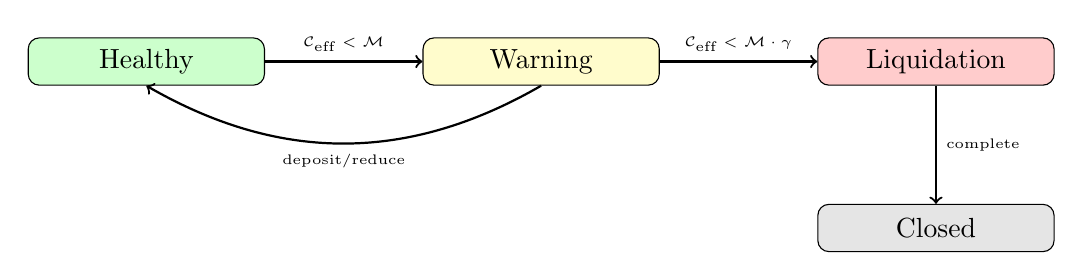
\begin{tikzpicture}[
    state/.style={rectangle, rounded corners, draw, minimum width=3cm, minimum height=0.6cm, align=center},
    arrow/.style={->, thick}
  ]
    \node[state, fill=green!20] (healthy) {Healthy};
    \node[state, fill=yellow!20, right=2cm of healthy] (warning) {Warning};
    \node[state, fill=red!20, right=2cm of warning] (liquidation) {Liquidation};
    \node[state, fill=gray!20, below=1.5cm of liquidation] (closed) {Closed};

    \draw[arrow] (healthy) -- node[above, font=\tiny] {$\mathcal{C}_{\text{eff}} < \mathcal{M}$} (warning);
    \draw[arrow] (warning) -- node[above, font=\tiny] {$\mathcal{C}_{\text{eff}} < \mathcal{M} \cdot \gamma$} (liquidation);
    \draw[arrow] (liquidation) -- node[right, font=\tiny] {complete} (closed);
    \draw[arrow, bend left] (warning.south) to node[below, font=\tiny] {deposit/reduce} (healthy.south);
  \end{tikzpicture}
  \caption{Account liquidation state machine. $\gamma$ is a liquidation threshold, typically $0.8$--$0.9$.}
  \label{fig:liquidation}
\end{figure}

The liquidation engine may:
\begin{itemize}
  \item \textbf{Standard liquidation:} Close positions against the public order book at market prices, distributing any forfeitable margin to liquidators and the insurance fund.
  \item \textbf{Backstop liquidation:} If the public book cannot absorb the liquidation without excessive slippage, route the position to a backstop liquidity pool composed of protocol-designated market makers, vaults, or the insurance fund.
  \item \textbf{Auto-deleveraging (ADL):} If the backstop is insufficient and the position would create bad debt, forcibly close the underwater position against profitable opposing positions at the bankruptcy price.
  \item \textbf{Contract unwind:} In an extreme tail event, a market may be paused and unwound pro-rata across participants.
\end{itemize}

This staged waterfall gives participants predictability, protects the broader protocol from one market's failure, and ensures that solvency enforcement can escalate with market stress.

\subsection{Insurance fund}

The insurance fund provides a buffer against liquidation deficits. It is funded by a portion of trading fees, liquidation penalties from underwater accounts, and optional LP-provided insurance capital earning a premium.

The fund is compartmentalized by market where practical, so that losses in one market do not automatically drain the global backstop. After market-level backstops are exhausted, a global insurance fund may be drawn upon. The global fund size target $F^*$ is determined by:
\[
F^* = \kappa \cdot \sqrt{\sum_{p \in \mathcal{P}_{\text{all}}} \text{size}_p^2}
\]
where $\kappa$ is a risk parameter to be calibrated against historical tail risk (Section~\ref{sec:economics}).

%=============================================================================
\section{Programmable Market Extensions}
\label{sec:markets}
%=============================================================================

Synchra defines a \textbf{market extension framework} that allows any financial primitive to be deployed as a clearing kernel extension. Extensions implement a canonical \texttt{IMarket} interface and expose lifecycle callbacks that the kernel invokes around position, funding, and liquidation events. This design adapts the hook-extensibility pattern to Arc's EVM environment and Synchra's clearing-kernel model.

The framework is intentionally permissive about execution semantics. An extension may use a public CLOB, an RFQ network, a batch auction, or a TEE-based matcher; the only requirement is that the resulting position changes and cash flows be settled through the kernel. This separation lets execution innovators compete on latency, privacy, and pricing while the kernel guarantees solvency.

\subsection{Extension interface}

Each market extension must implement the \texttt{IMarket} interface (Algorithm~\ref{alg:market}) and expose the following lifecycle callbacks:

\begin{figure}[h]
  \caption{Market extension lifecycle callbacks}
  \label{alg:hooks}
  \begin{quote}
  \texttt{\textbf{callback} beforeOpenPosition(user, market, size, price)} \\
  \texttt{\textbf{callback} afterOpenPosition(user, market, position)} \\
  \texttt{\textbf{callback} beforeClosePosition(user, market, position)} \\
  \texttt{\textbf{callback} afterClosePosition(user, market, pnl)} \\
  \texttt{\textbf{callback} beforeSettleFunding(market, rate)} \\
  \texttt{\textbf{callback} onLiquidation(user, market, position)} \\
  \texttt{\textbf{callback} onOracleUpdate(market, price)}
  \end{quote}
\end{figure}

Extensions are stateless with respect to the kernel -- they may maintain their own state (e.g., funding accumulators, LP shares) but must deterministically settle through the kernel.

\subsection{Privacy-preserving perpetual module}

The perpetual module implements standard BTC/ETH perpetuals with configurable privacy:
\begin{itemize}
  \item \textbf{Funding rate:} computed continuously from a per-market funding index, so that funding payments are independent of the exact settlement block:
  \[
  \Delta F_t = \text{clamp}\left(\frac{P_{\text{mark}} - P_{\text{index}}}{P_{\text{index}}}, -\text{max\_rate}, +\text{max\_rate}\right) \cdot \Delta t
  \]
  where $\Delta t$ is the time elapsed since the last index update. A position's funding PnL is computed lazily as $Q \cdot (F_{\text{current}} - F_{\text{entry}}) \cdot P_{\text{index}}$.
  \item \textbf{Mark price:} median of external feeds, on-chain impact mid-price, basis-adjusted fair value, and best bid/ask/last trade, clamped tightly to the oracle index price to resist manipulation.
  \item \textbf{Leverage:} 1x--50x market-level ceiling, adjustable by risk tier; effective account leverage is computed by the portfolio risk engine, not read from a single position (Section~\ref{sec:clearing}).
  \item \textbf{Liquidation:} Maintenance margin at 50\%--75\% of initial margin, adjusted by portfolio risk.
  \item \textbf{Private mode:} Takers may route orders through the encrypted orderbook, preventing leakage of size and position direction.
\end{itemize}

\subsection{FX perpetual module}

The FX module enables trading of currency pairs:
\begin{itemize}
  \item \textbf{Pairs:} EURC/USDC, GBP/USD, JPY/USD (with appropriate settlement assets).
  \item \textbf{StableFX integration:} FX positions settled in USDC use CCTP-based conversion at settlement time, removing the need for deep EURC/USDC LPs and aligning with Circle's programmable FX vision.
  \item \textbf{Funding:} Interest rate differential-based funding reflecting the carry trade:
  \[
  r_{\text{FX}} = r_{\text{quote}} - r_{\text{base}}
  \]
  \item \textbf{Hedging utility:} Enterprises receiving EURC can hedge FX exposure without leaving the Arc ecosystem.
\end{itemize}

\subsection{Tokenized RWA and rate module}

Real-world asset derivatives and rate exposures:
\begin{itemize}
  \item \textbf{Underlyings:} Tokenized money-market yields (USYC), treasury yields, gold, credit indices.
  \item \textbf{Pricing:} Oracle-driven with redundant feeds and circuit breakers.
  \item \textbf{Settlement:} Cash-settled in USDC -- no physical delivery.
  \item \textbf{Yield trading:} Users can trade exposure to USYC yield, SOFR-like rates, or Treasury yields as synthetic instruments, hedging rate risk within the same portfolio.
\end{itemize}

\subsection{Strategy vault module}

Strategy vaults are deployed as market extensions that trade through the kernel on behalf of depositors (full details in Section~\ref{sec:yield}). The module exposes:
\begin{itemize}
  \item \textbf{Vault registration:} a vault declares its strategy rule set, allowed markets, leverage bounds, and performance fee.
  \item \textbf{Execution callbacks:} the kernel calls vault-defined position-adjustment logic at rebalance triggers.
  \item \textbf{Risk isolation:} each vault has its own sub-account and portfolio margin, protecting other kernel participants from vault-specific strategy failures.
\end{itemize}

\subsection{Repo and basis module}

A repo market extension allows collateralized borrowing and lending within the kernel:
\begin{itemize}
  \item \textbf{Secured loans:} borrowers post eligible collateral and receive USDC/USYC against a haircut.
  \item \textbf{Term and overnight repo:} configurable maturity, with rates set by an order-driven funding market.
  \item \textbf{Integration:} repo loans are liabilities and repo deposits are assets within portfolio margin, enabling basis-trade vaults and treasury-collateralized leverage.
\end{itemize}

%=============================================================================
\section{Execution Layer}
\label{sec:execution}
%=============================================================================

The execution layer provides multiple execution modes to accommodate different market requirements and privacy preferences.

\subsection{Public CLOB}

The public central-limit-order-book extension supports transparent, liquid markets. It is designed with gas efficiency as a first-class constraint: post, cancel, and modify operations should be storage-light so that market makers can update quotes frequently without paying prohibitive gas. Synchra uses compact, finance-optimized data structures for price-level discovery and order storage, with a single-transaction modify operation that moves an order's storage slot rather than deleting and re-creating it.

Orders are matched by price-time priority. The matching engine validates signatures, maintains the order book, and submits matched trades to the kernel as settlement batches. The matching engine is trusted for sequencing but not for correctness: all fills are independently verifiable against the signed order set.

\subsection{Request-for-quote (RFQ)}

For block trades and institutional orders, the RFQ system:
\begin{enumerate}
  \item A taker broadcasts an RFQ specifying market, side, and size (optionally with price limits).
  \item Market makers respond with quotes within a time window.
  \item The taker selects a quote, and the trade settles atomically.
  \item Failed RFQs (no quotes, expired quotes) have no onchain effect.
\end{enumerate}

\subsection{Batch auctions}

To mitigate MEV, frequent batch auctions (FBAs) are supported:
\begin{enumerate}
  \item Orders are collected during an accumulation period (typically 1--5 seconds).
  \item At the close, a uniform clearing price is computed that maximizes matched volume.
  \item All trades execute at the clearing price, eliminating priority gas auction (PGA) advantages.
\end{enumerate}

The clearing price $p^*$ for a batch with bids $\{b_i\}$ and asks $\{a_j\}$ satisfies:
\[
p^* = \arg\max_{p} \min\left(\sum_{i} \text{vol}_i \cdot \mathbf{1}_{b_i \geq p}, \sum_{j} \text{vol}_j \cdot \mathbf{1}_{a_j \leq p}\right)
\]

%=============================================================================
\section{Privacy Architecture}
\label{sec:privacy}
%=============================================================================

Synchra provides a layered privacy model where users choose their confidentiality level per order or per position.

\subsection{Privacy dimensions}

Users may conceal:

\begin{enumerate}
  \item \textbf{Order intent:} The price, size, side, and market of an order are encrypted until execution.
  \item \textbf{Position size:} The notional exposure of open positions is hidden from other participants.
  \item \textbf{Leverage:} The leverage multiplier is private.
  \item \textbf{PnL:} Realized and unrealized profit/loss is hidden.
  \item \textbf{Portfolio exposure:} The composition of the collateral pool and open positions across markets is concealed.
\end{enumerate}

\subsection{Privacy modes}

\begin{table}[h]
  \centering
  \begin{tabular}{lll}
    \toprule
    \textbf{Mode} & \textbf{Visibility} & \textbf{Use case} \\
    \midrule
    Public & All order parameters visible & Retail, liquid markets \\
    Protected & Order parameters visible, identity hidden & Whales, institutions \\
    Confidential & Encrypted orders, TEE matching & Large block trades \\
    Selective & Partial disclosure via ZK & Solvency attestation \\
    \bottomrule
  \end{tabular}
  \caption{Privacy modes available to Synchra users.}
  \label{tab:privacy}
\end{table}

\subsection{Private order flow}

Confidential orders follow a commit-reveal flow:

\begin{enumerate}
  \item The trader submits a commitment $H(\text{order}, r)$ where $r$ is a random nonce.
  \item At the execution deadline, the trader reveals $(\text{order}, r)$.
  \item The execution engine verifies the commitment, matches the order, and settles.
  \item If the trader fails to reveal, the order is treated as canceled; the commitment expires.
\end{enumerate}

For continuous execution, orders are submitted directly to the TEE matcher.

%=============================================================================
\section{Trusted Execution Environment}
\label{sec:tee}
%=============================================================================

TEEs provide a practical middle ground between fully transparent and fully private execution, offering confidentiality with hardware-level trust.

\subsection{TEE architecture}

\begin{figure}[h]
  \centering
  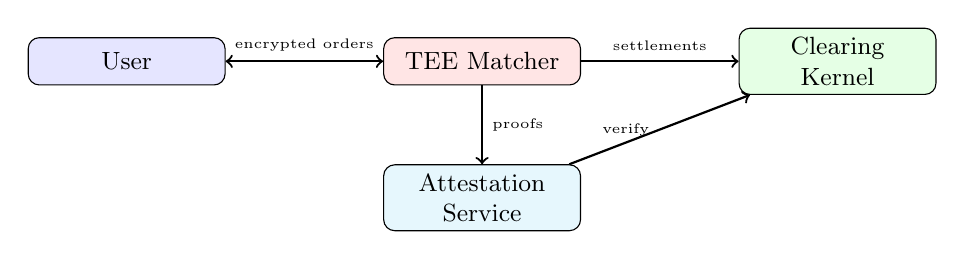
\begin{tikzpicture}[
    comp/.style={rectangle, draw, rounded corners, minimum width=2.5cm, minimum height=0.6cm, align=center, font=\small},
    arrow/.style={->, thick},
    doublearrow/.style={<->, thick}
  ]
    \node[comp, fill=blue!10] (user) {User};
    \node[comp, fill=red!10, right=2cm of user] (tee) {TEE Matcher};
    \node[comp, fill=green!10, right=2cm of tee] (kernel) {Clearing\\Kernel};
    \node[comp, fill=cyan!10, below=1cm of tee] (attest) {Attestation\\Service};

    \draw[doublearrow] (user) -- node[above, font=\tiny] {encrypted orders} (tee);
    \draw[arrow] (tee) -- node[above, font=\tiny] {settlements} (kernel);
    \draw[arrow] (tee) -- node[right, font=\tiny] {proofs} (attest);
    \draw[arrow] (attest) -- node[left, font=\tiny] {verify} (kernel);
  \end{tikzpicture}
  \caption{TEE-based execution flow.}
  \label{fig:tee}
\end{figure}

\textbf{Order submission:} Users encrypt orders with the TEE's public key. The TEE decrypts within the enclave, ensuring plaintext never leaves the hardware boundary.

\textbf{Matching:} The TEE matcher processes orders with access to the full order book. Matching logic is identical to the public CLOB but operates on decrypted orders.

\textbf{Attestation:} The TEE produces a signed attestation of each match, proving correct execution within the enclave. Attestation is verified on-chain before settlement.

\textbf{Fallbacks:} If the TEE is compromised (attestation verification fails), the system falls back to on-chain settlement with public execution.

\subsection{TEE security model}

\begin{itemize}
  \item \textbf{Trust assumption:} The hardware manufacturer (Intel/AMD) is honest. We assume TDX and SEV-SNP provide memory isolation and attestation integrity.
  \item \textbf{Mitigation:} Multiple independent enclave implementations reduce single-vendor risk.
  \item \textbf{Limitation:} Side-channel attacks (cache timing, power analysis) are acknowledged but considered out of scope for the current threat model.
\end{itemize}

%=============================================================================
\section{Zero-Knowledge Layer}
\label{sec:zk}
%=============================================================================

ZK proofs are used selectively for specific high-value operations where proof of correctness is required without revealing the underlying data. We explicitly do not use ZK for per-order matching or execution, as the latency and cost of proof generation make it impractical for high-frequency trading. Instead, ZK is applied where it provides the greatest marginal value: solvency attestation, periodic batch verification, and TEE attestation verification.

\subsection{Solvency proof}

Institutions and agents can periodically prove solvency without revealing positions:

\[
\pi_{\text{solvent}} : \text{Prove}\left( \sum_{a \in \mathcal{A}} \text{collateral}_a > \sum_{p \in \mathcal{P}} \text{liability}_p \right)
\]

This enables transparent solvency reporting -- a requirement for regulated institutions -- without portfolio disclosure. The proof is generated off-chain by the institution and verified on-chain, allowing anyone to confirm that an account is solvent without learning its composition or size.

\subsection{Periodic batch verification}

For non-continuous verification, a matching engine can periodically produce a ZK proof that a batch of settlements was computed correctly:

\[
\pi_{\text{batch}} : \text{Prove}\left( \forall t \in \mathcal{T}_{\text{batch}}: \text{settlement}_t = f(\text{order}_t, \text{state}_t) \right)
\]

This proof is generated at discrete intervals (e.g., hourly) rather than per-order, amortizing the proving cost across many trades. The verification contract confirms correctness without re-executing the match logic.

\subsection{ZK for TEE attestation verification}

Following the approach demonstrated by Kalypso~\cite{marlin_kalypso}, we use ZK proofs to compress TEE attestation verification. Verifying an Intel TDX or AMD SEV-SNP attestation certificate directly on-chain costs approximately 75M gas. By generating a ZK proof that the attestation is valid, this cost is reduced to roughly 300K gas -- a factor of 200x improvement. This is applied as a defense-in-depth layer: the TEE provides execution privacy, and the ZK-compressed attestation provides verifiable integrity at practical cost.

\subsection{Implementation}

For solvency and batch proofs, the ZK suite uses:
\begin{itemize}
  \item \textbf{Backend:} Arkworks (Rust) for constraint generation.
  \item \textbf{Constraint system:} R1CS.
  \item \textbf{Proof system:} Groth16 with BN254 curve.
  \item \textbf{Verification:} Solidity verifier contracts deployed on Arc EVM.
\end{itemize}

\subsection{Limitations}

\begin{itemize}
  \item Groth16 requires a trusted setup per circuit. We use a multi-party ceremony.
  \item Proof generation cost limits ZK application to low-frequency, high-value operations (solvency attestations, hourly batch verification). For per-order privacy, TEE execution or commit-reveal protocols are preferred.
  \item Recursive proofs may be used to aggregate multiple solvency attestations into a single proof for scaling.
\end{itemize}

%=============================================================================
\section{Agent-Native Financial Markets}
\label{sec:agents}
%=============================================================================

Synchra treats autonomous agents as first-class protocol participants, not as scripts operated by indirectly authorized traders.

\subsection{Agent accounts}

An agent account extends the standard clearing account with:

\begin{itemize}
  \item \textbf{Cryptographic identity:} The agent has a native key pair, registered on-chain.
  \item \textbf{Permission model:} Fine-grained permissions encoded as a capability token, signed by the account owner's registered key over the scoped action fields:
  \[
  \text{capability} = \text{Sign}_{sk_{\text{owner}}}\big(H(\text{agent\_id}, \text{action}, \text{limits}, \text{expiry})\big)
  \]
  The kernel verifies the signature against the account's registered owner key before honoring any action authorized under the capability; the hash alone identifies the scoped grant, and the signature is what makes it enforceable and non-forgeable.
  \item \textbf{Execution policy:} Constraints on what the agent can do, enforced at the kernel level:
  \begin{itemize}
    \item Maximum position size per market.
    \item Maximum leverage.
    \item Allowed market types.
    \item Daily loss limits.
    \item Cooldown periods between actions.
  \end{itemize}
  \item \textbf{Session keys:} Ephemeral keys with limited scope and expiry, allowing agents to operate without exposing the master key.
  \item \textbf{Nanopayments integration:} Agents use Circle's Nanopayments~\cite{circle_nanopayments} for gas-free sub-cent USDC transfers, enabling high-frequency, low-value transactions such as API payments, streaming data fees, and per-compute-unit billing that would be uneconomical on traditional payment rails.
  \item \textbf{Agent Stack compatibility:} Agent accounts are designed to integrate with Circle's Agent Stack~\cite{circle_agent_stack}, providing a standard interface for connecting AI models to wallet infrastructure, payment authorization, and onchain settlement.
\end{itemize}

\subsection{Agent types}

\begin{description}
  \item[Trading agents] Execute strategies with configurable risk parameters. Trading agents are constrained by the portfolio margin engine -- they cannot open positions that would violate the account's risk limits.
  \item[Treasury agents] Manage hedging, yield optimization, and FX exposure for institutions. A treasury agent might maintain a delta-neutral BTC position while earning funding, or hedge EURC-denominated liabilities.
  \item[Liquidity agents] Provide two-sided quotes in RFQ markets. Liquidity agents implement market-making strategies and are compensated through the spread.
  \item[Research agents] Aggregate information and reflect it in prediction or event-derivative markets. Research agents are the information backbone of the event-derivatives ecosystem.
\end{description}

\subsection{Agent security}

Agent compromise is mitigated by:
\begin{itemize}
  \item \textbf{Principle of least privilege:} Each agent capability is narrowly scoped.
  \item \textbf{Circuit breakers:} Agents have programmable spending and loss limits.
  \item \textbf{Session expiry:} Keys are ephemeral and must be periodically refreshed.
  \item \textbf{Revocation:} The account owner can revoke any agent capability at any time.
  \item \textbf{Anomaly detection:} Off-chain monitoring systems flag unusual agent behavior.
\end{itemize}

%=============================================================================
\section{Yield and Strategy Vaults}
\label{sec:yield}
%=============================================================================

A clearing layer that merely holds collateral is capital inefficient. Synchra treats idle collateral as productive capital: it earns yield while simultaneously backing positions, and it can be deployed into programmatic strategies that themselves trade through the kernel. This section formalizes the yield-bearing collateral tiers and the programmable strategy vault framework.

\subsection{Yield-bearing collateral tiers}

Synchra's collateral tiers are exactly the four tiers introduced in Table~\ref{tab:collateral} (Section~\ref{sec:clearing}); this section describes how each tier accrues yield. Cross-chain origin is \emph{not} a separate tier: an asset bridged via CCTP retains its base tier classification and simply carries the cross-chain haircut modifier noted in Table~\ref{tab:collateral}.

\begin{description}
  \item[Tier 1 (USDC, EURC).] Instant settlement with Arc's native stablecoins. Depositors may opt into a sweep module that routes idle Tier-1 balances into overnight repo or money-market instruments, earning a baseline yield while preserving same-block liquidity for margin calls.
  \item[Tier 2 (USYC, stUSD).] USYC is a tokenized representation of a regulated money-market fund and is already a yield-bearing asset~\cite{usyc}. Held as Tier-2 collateral, USYC contributes its fund yield to the depositor and receives a reduced haircut due to its high credit quality and liquidity.
  \item[Tier 3 (ETH, BTC liquid staking).] Liquid staking derivatives accrue native staking yield while posted as collateral, subject to the higher haircut reflecting price volatility and slashing risk relative to Tiers 1--2.
  \item[Tier 4 (tokenized RWAs).] Longer-duration tokenized Treasuries, repo instruments, or credit products earn higher yield but carry higher haircut and liquidity constraints. Tier-4 collateral is marked through independent oracles and subject to stress-based haircuts.
\end{description}

\textbf{Cross-chain modifier.} USDC, EURC, or USYC bridged via CCTP from another chain retains the base-tier treatment above (Tier 1 or Tier 2 respectively) but is subject to the additional haircut increment specified in Table~\ref{tab:collateral}, reflecting bridging and rebalancing latency rather than a distinct risk class.

\textbf{Yield attribution.} Each collateral asset accrues its native yield to the depositor's account, net of any protocol keep fee (typically 0--10 bps). The yield is computed continuously and can be reinvested or withdrawn subject to margin requirements. Importantly, yield accrual does not reduce the collateral's eligibility for margin; the asset's value for margin purposes is its market value plus accrued yield.

\subsection{Programmable strategy vaults}

Strategy vaults are smart-contract-managed sub-accounts that execute predefined strategies through the Synchra kernel. They are first-class participants: each vault has its own account, collateral allocation, risk limits, and position set, all governed by the same clearing kernel.

\textbf{Vault mechanics.} A strategy vault:
\begin{enumerate}
  \item receives deposits from users in approved collateral assets;
  \item allocates capital across one or more market extensions according to a strategy rule set;
  \item opens leveraged positions through the kernel, subject to the vault's own portfolio margin;
  \item accrues trading PnL, funding payments, and collateral yield;
  \item periodically rebalances and distributes returns to depositors, net of a performance fee.
\end{enumerate}

Because vaults trade through the unified kernel, they benefit from the same cross-market margin and privacy options as individual traders. A single vault can simultaneously run a delta-neutral ETH perpetual basis trade, an FX carry position, and a tokenized-Treasury repo leg -- all margined together.

\subsection{Example strategies}

\begin{description}
  \item[Delta-neutral market-making vault.] Provides liquidity on the public CLOB while hedging directional exposure externally. Earns maker fees plus USYC yield on unused collateral.
  \item[Basis trading vault.] Long spot / short perp (or vice versa) to capture funding-rate premiums. Cross-market margin allows the spot collateral to back the short perpetual.
  \item[FX-hedged RWA carry vault.] Holds tokenized Treasuries or credit products while shorting the relevant FX exposure through the FX perpetual module.
  \item[Funding-rate arbitrage vault.] Shorts an over-funded perpetual and longs an under-funded perpetual on correlated markets, capturing funding-rate differentials with offsetting notional.
  \item[Collateral transformation / repo vault.] Lends idle Tier-2/Tier-4 collateral into the repo module and borrows USDC against it, earning the repo spread while keeping liquidity available for margin.
  \item[Privacy-preserving block-trade vault.] Aggregates large-size flow through encrypted RFQs and executes via TEE matching, then clears through the kernel.
  \item[Smart treasury vault.] An enterprise or agent deposits EURC/USDC receipts and automatically hedges FX and rate exposure via programmable policies, rebalancing as invoices or obligations settle.
\end{description}

\subsection{Repo and securities lending module}

To further increase capital efficiency, Synchra supports an internal repo market:
\begin{itemize}
  \item Lenders post idle Tier-2/Tier-4 collateral into a repo pool and earn interest from borrowers.
  \item Borrowers post eligible collateral and receive a loan of the same or different asset, with haircuts and term structures enforced by the kernel.
  \item Repo positions are integrated into portfolio margin: a repo loan is a liability; a repo deposit is an asset, both marked at market.
  \item Liquidation of repo positions follows the same auction mechanism as derivative positions.
\end{itemize}

This module turns Synchra into a tri-party-style collateral management system: collateral can be borrowed, lent, margined, and yield-bearing within a single risk framework.

\subsection{Structured product vaults}

Synchra's modular design supports structured products issued as vaults:
\begin{itemize}
  \item \textbf{Principal-protected yield notes:} combine a zero-coupon tokenized Treasury with a small options position.
  \item \textbf{Range accruals:} earn enhanced yield if EURC/USDC trades within a range, using FX perpetuals for delta hedging.
  \item \textbf{Autocallables:} knock-in/knock-out structures backed by perp and RWA positions.
\end{itemize}

Each structured product is simply a vault with a custom strategy rule set and a defined payoff function. The clearing kernel handles the margin, settlement, and liquidation logic uniformly. These are the instruments referenced in Section~\ref{sec:clearing} as carrying an upfront premium at trade settlement.

%=============================================================================
\section{Economic Model}
\label{sec:economics}
%=============================================================================

Synchra has no protocol token. Value accrues to depositors, liquidity providers, strategy vault managers, and the protocol treasury through fee revenue and yield-bearing collateral. This model aligns incentives without introducing speculative token dynamics or regulatory ambiguity.

\subsection{Fee structure}

Synchra charges fees at multiple points:

\begin{table}[h]
  \centering
  \begin{tabular}{lll}
    \toprule
    \textbf{Fee type} & \textbf{Rate} & \textbf{Beneficiary} \\
    \midrule
    Trading fee (maker) & 0\%--0.02\% & Liquidity providers \\
    Trading fee (taker) & 0.03\%--0.06\% & Liquidity providers, protocol treasury \\
    Funding (perp) & Variable & Long/short transfer \\
    Order recycle fee & Configurable & Participant who removes expired order \\
    Withdrawal fee & 0\%--0.01\% & Protocol treasury \\
    Strategy vault performance fee & 10\%--20\% & Vault manager, protocol treasury \\
    Yield keep fee & 0\%--10 bps & Protocol treasury \\
    Repo spread & 10\%--25\% of interest & Protocol treasury, insurance fund \\
    Liquidation penalty & 1\%--5\% & Liquidator, insurance fund \\
    \bottomrule
  \end{tabular}
  \caption{Synchra fee schedule. Rates are dynamic based on market conditions and volume tiers.}
  \label{tab:fees}
\end{table}

\textbf{Order recycle fees.} Orders submitted with an expiry block must attach a small recycle fee. The fee is refunded if the order fills or the issuer cancels it. If the order expires, the first participant who encounters the expired order during book traversal may claim the recycle fee as compensation for removing stale state. This economic cleanup incentive keeps the order book compact and rewards participants for protocol hygiene.

\subsection{Protocol sustainability}

Revenue from trading fees, vault performance fees, yield keep fees, and repo spreads funds:
\begin{itemize}
  \item Insurance fund growth and backstop capital.
  \item Security audits, formal verification, and bug bounties.
  \item TEE infrastructure and oracle costs.
  \item Liquidity incentives during bootstrapping (paid in USDC/EURC, not a token).
  \item Protocol development and governance operations.
\end{itemize}

Because Synchra does not issue a token, all incentives are paid in stablecoins or yield-bearing assets. This eliminates the need for inflationary emissions, aligns the protocol with Arc's stablecoin-native thesis, and simplifies regulatory treatment. The tradeoff is that Synchra cannot bootstrap early liquidity with speculative token emissions the way many competing protocols do; early LP and insurance capital must instead be attracted with real fee yield, USYC-denominated incentive programs funded from the protocol treasury, and design choices (deep cross-market margin, privacy) that are difficult for token-incentivized competitors to replicate quickly.

\subsection{Economic security}

The protocol's economic security relies on:

\textbf{Collateral adequacy.} Portfolio margin ensures that collateral requirements reflect actual portfolio risk. Scenario parameters will be calibrated against major historical volatility events (e.g., May 2021, the LUNA collapse, November 2022) as part of the risk engine's pre-launch validation, with backtesting results published ahead of mainnet deployment.

\textbf{Liquidation robustness.} The multi-stage liquidation process prevents cascading failures. Partial liquidation allows orderly position reduction before forced closure.

\textbf{Insurance fund.} The dynamic fund size target $F^*$ is designed to scale with market risk. Initial calibration will target 99.5\% coverage under historically observed price movements, to be validated through backtesting prior to mainnet deployment rather than assumed.

\textbf{Liquidity provider diversification.} Risks are distributed across LPs who have heterogeneous risk preferences and can exit according to their liquidity terms.

\subsection{Incentive alignment}

LP and insurance capital is subject to minimum lockup periods (configurable per pool, typically 7--30 days) to prevent hot-money flows. Returns are proportional to risk assumed, measured by the VaR contribution of capital to each market. Strategy vault managers earn performance fees only on positive returns, aligning their interests with depositors.

\subsection{Value proposition}

For depositors, Synchra offers:
\begin{itemize}
  \item \textbf{Yield on collateral:} USYC, repo, and sweep yields accrue while assets back positions.
  \item \textbf{Leverage:} portfolio margin allows more exposure per dollar of collateral than isolated-margin alternatives.
  \item \textbf{Privacy:} encrypted execution protects large order flow and strategy leakage.
  \item \textbf{Composability:} one pool of capital serves FX, perpetuals, RWA, and strategy vaults.
\end{itemize}

For the Arc ecosystem, Synchra increases capital velocity, deepens liquidity across all market extensions, and provides the institutional-grade clearing infrastructure that complex financial applications require.

%=============================================================================
\section{Arc Ecosystem Alignment}
\label{sec:arc}
%=============================================================================

Synchra is designed from the ground up for deployment on Circle's Arc blockchain~\cite{circlearc}, leveraging the full Circle developer platform for settlement, collateral, and agent infrastructure.

\subsection{Alignment with Arc's philosophy}

Circle describes Arc as the foundation for an open, stablecoin-native financial system. Its public priorities include:
\begin{itemize}
  \item \textbf{Stablecoin-native finance:} USDC and EURC as settlement rails, with USDC as native gas.
  \item \textbf{Programmable FX and cross-border payments:} real-time, programmable currency exchange and settlement.
  \item \textbf{Tokenized real-world assets:} money-market funds, Treasuries, and credit products composable with onchain markets.
  \item \textbf{Autonomous agents and smart treasuries:} AI-driven participants managing payment, hedging, and investment workflows.
  \item \textbf{Institutional-grade trust and compliance:} deterministic finality, permissioned/permissionless options, and privacy-preserving infrastructure.
\end{itemize}

Synchra directly advances each of these priorities. Its clearing kernel is stablecoin-native; its FX perpetual and cross-currency margin modules make programmable FX economically viable; its USYC and RWA collateral tiers turn tokenized assets into productive margin; its agent accounts and strategy vaults enable smart treasuries; and its privacy architecture provides the confidentiality that institutional flow requires. Synchra does not add generic DeFi to Arc -- it builds the specific market infrastructure Arc's own thesis calls for.

\subsection{Filling Arc's infrastructure gaps}

The Arc ecosystem today has strong foundations in swaps, payments, and lending, but every category that requires cross-market coordination, privacy, or composable risk management remains underdeveloped. Synchra is purpose-built to fill these gaps.

The clearing kernel provides the cross-market infrastructure that no individual exchange can justify building. The modular extension framework allows perpetuals, FX derivatives, RWA markets, and programmable strategy vaults to share a unified collateral pool and risk engine on Arc -- an architecture that is rare on any chain and absent from the current Arc ecosystem. The privacy modes (Section~\ref{sec:privacy}) bring confidential execution to Arc as an application-layer complement to its protocol-level privacy roadmap. The agent-native architecture (Section~\ref{sec:agents}) and yield/strategy vault framework (Section~\ref{sec:yield}) integrate with Circle's Agent Stack, USYC, and Nanopayments -- the products Circle is actively prioritizing for the Arc developer ecosystem.

Synchra does not compete with other Arc protocols. It provides the infrastructure layer that makes their markets more capital-efficient. A lending protocol on Arc using Synchra can margin its lending positions against perpetual positions. A programmable FX protocol on Arc can settle through Synchra's clearing kernel. Synchra is infrastructure, not isolation.

\subsection{Stablecoin-native settlement}

Arc's defining architectural choice -- using USDC as its native gas token -- aligns directly with Synchra's settlement model. All collateral, margin, fee, and PnL flows in Synchra are denominated in stablecoins (USDC, EURC), eliminating the dual-volatility problem present in protocols where users must manage both position risk and gas token price risk. Arc's deterministic sub-second finality enables the real-time settlement that portfolio margin requires, where rapid position updates must be reflected in collateral availability.

\subsection{Tokenized collateral via USYC}

USYC~\cite{circle_usyc}, Circle's tokenized money market fund, serves as yield-bearing collateral within Synchra's collateral engine (Tier 2, Section~\ref{sec:clearing}). This allows traders to earn yield on idle collateral while maintaining the ability to open and close positions -- a capability not available in protocols limited to non-yield-bearing stablecoin collateral.

\subsection{Nanopayments for agent-to-agent settlement}

Circle's Nanopayments~\cite{circle_nanopayments} enable gas-free sub-cent USDC transfers, which are critical for the agent-native architecture (Section~\ref{sec:agents}). Agents performing high-frequency, low-value transactions -- API calls, streaming data purchases, per-compute-unit billing -- would be uneconomical at standard gas costs. Nanopayments, powered by Circle Gateway, batch these microtransactions and settle them as aggregated onchain transfers, making agent-to-agent micropayments viable at scale.

\subsection{Agent Stack integration}

Circle's Agent Stack~\cite{circle_agent_stack} provides a standard framework for connecting AI models to wallet infrastructure, payment authorization, and onchain settlement. Synchra's agent account model (Section~\ref{sec:agents}) is designed to be compatible with this stack, allowing developers to deploy agents that use Circle's programmable wallets for custody and Synchra's clearing kernel for trading and treasury management, within a unified permission model.

\subsection{CCTP interoperability}

Circle's Cross-Chain Transfer Protocol~\cite{cctp} enables USDC transfers across supported blockchains, allowing Synchra to accept collateral originating from other networks without fragmented liquidity. This is particularly important for institutional participants who may hold USDC across multiple chains and require unified treasury management.

\subsection{Restricted product access}

Some Arc ecosystem products relevant to Synchra -- StableFX, USYC, and Circle Payments Network -- are currently permissioned enterprise products. Synchra's architecture accommodates this by treating these integrations as optional enterprise features, with core protocol functionality operating on permissionless primitives (USDC, EURC, Arc EVM).

%=============================================================================
\section{Security Analysis}
\label{sec:security}
%=============================================================================

\subsection{Oracle manipulation}

Synchra uses a multi-oracle architecture:
\begin{itemize}
  \item \textbf{Primary oracle:} Pyth Network for real-time price feeds.
  \item \textbf{Secondary oracle:} Chainlink for staleness checks.
  \item \textbf{Tertiary oracle:} TWAP from CLOB trades for circuit breaker comparison.
\end{itemize}

If the primary and secondary oracles diverge by more than $\delta$ (configurable, typically 1\%--5\%), a circuit breaker pauses market operations until convergence is restored.

For event-derivative and oracle-dependent markets, resolution uses a dispute window with bond-based challenges.

\subsection{Liquidation cascades}

Portfolio margin can create correlated liquidations during market stress. Mitigations include:
\begin{itemize}
  \item \textbf{Gradual liquidation:} Positions are liquidated in tranches rather than all at once.
  \item \textbf{Liquidation queue:} Liquidations are ordered by time of distress, not all executed simultaneously.
  \item \textbf{Circuit breaker:} If the total liquidation volume exceeds a threshold within a window, trading is paused.
\end{itemize}

\subsection{Smart contract risk}

The clearing kernel is designed to be formally verified. Key invariants:
\begin{itemize}
  \item Collateral cannot be created or destroyed outside of authorized operations.
  \item Position modifications are atomic with collateral updates.
  \item Settlement is deterministic given the same input state.
  \item Market extensions cannot manipulate kernel state outside their authorized interfaces.
\end{itemize}

\subsection{Privacy assumptions}

\begin{itemize}
  \item TEE assumes hardware security. Compromise would reveal encrypted order flow but not alter settlement.
  \item Commit-reveal assumes the reveal phase is incentivized (bonding).
  \item Metadata leakage (order frequency, timing, network-level patterns) is acknowledged as out of scope.
\end{itemize}

\subsection{ZK assumptions}

\begin{itemize}
  \item ZK proofs are used only for low-frequency operations (solvency attestation, batch verification, TEE attestation compression), not per-order execution.
  \item Groth16 requires a trusted setup per circuit. We use a multi-party ceremony.
  \item Proof generation cost, while non-trivial, is amortized across many trades in batch verification or across reporting periods for solvency attestation.
\end{itemize}

%=============================================================================
\section{Related Work}
\label{sec:related}
%=============================================================================

Synchra builds on decades of work in derivatives clearing, portfolio margin, private execution, modular exchange design, and tokenized yield infrastructure. This section situates the design without naming individual competing protocols.

\subsection{Orderbook and liquidity-pool derivatives}

Onchain derivatives have evolved through three broad generations. First-generation protocols used virtual AMMs for price discovery, inheriting liquidity limitations from spot AMMs. Second-generation protocols introduced pooled-collateral models, enabling deep markets without orderbooks but concentrating risk in liquidity providers. Third-generation protocols moved to orderbook-based execution on dedicated infrastructure, demonstrating that onchain CLOBs can match centralized exchange latency when execution and settlement are designed together. Synchra's clearing kernel is agnostic to the execution model above it: it can settle trades from public CLOBs, RFQs, batch auctions, or TEE-based matching.

\subsection{Layer separation and specialization}

A persistent lesson from modern exchange design is that clearing, risk, and execution should be separated. Specialized clearing layers can remain market-agnostic while execution layers compete on speed, privacy, and pricing. Some designs push this further by separating matching into geographically distributed zones near the source of spot price discovery. Synchra adapts the separation principle to Arc: the clearing kernel and margin engine are unified and on-chain, while execution can be public, encrypted, or batched depending on the market. Arc's deterministic sub-second finality removes the need for custom consensus clusters or physical colocation; Synchra's "colocation" is native integration with Arc's USDC/EURC/USYC settlement, CCTP, and Agent Stack.

\subsection{Portfolio margin}

Traditional clearing houses developed portfolio margining over decades, with SPAN and STANS as industry-standard models. A few onchain protocols have introduced portfolio margin concepts within single asset classes. Synchra extends this approach to heterogeneous market types -- perpetuals, FX derivatives, RWA markets, and strategy vaults -- through a unified clearing kernel.

\subsection{Modular exchange architectures}

Recent exchange designs have shown the power of modular extensibility: hooks that run custom logic around lifecycle events, separated clearing and execution layers, and per-market configuration. Synchra adopts this philosophy at the clearing layer: market extensions implement lifecycle callbacks around position, funding, and liquidation events, operating on clearing state rather than swap state.

\subsection{Private execution}

Private onchain execution has been explored through zero-knowledge proofs, multi-party computation, and trusted execution environments. Each approach involves tradeoffs: ZK provides strong confidentiality guarantees but can introduce latency and cost that limit high-frequency use; TEE-based matching offers lower latency but requires attestation and hardware trust assumptions; batch auctions mitigate MEV without hiding positions. Synchra takes a layered approach: TEE-based execution for latency-sensitive matching, with ZK reserved for higher-level verification tasks such as solvency attestation, batch correctness, and TEE attestation compression.

\subsection{Tokenized yield and agent infrastructure}

The emergence of tokenized money-market funds as yield-bearing collateral, gas-free micropayment rails, and agent-oriented wallet infrastructure creates the conditions for autonomous treasury and trading agents. Synchra integrates these primitives directly into its clearing kernel: yield-bearing collateral tiers earn while backing positions, and agent accounts operate with programmable policies, session keys, and micropayment support.

%=============================================================================
\section{Implementation Roadmap}
\label{sec:roadmap}
%=============================================================================

\subsection{Accelerator MVP: privacy-preserving BTC/USDC perpetual on Arc Testnet}

The initial build targets a focused, high-quality demonstration that validates the three moats and creates the foundation for the full accelerator program:

\begin{itemize}
  \item \textbf{Leverage:} clearing kernel with isolated margin, liquidation waterfall, and a single BTC/USDC perpetual extension.
  \item \textbf{Privacy:} encrypted RFQ flow for size orders with TEE-based quote matching.
  \item \textbf{Programmable yield:} USYC as an eligible collateral tier earning yield while backing positions.
\end{itemize}

\textbf{Deliverables:}
\begin{itemize}
  \item Clearing kernel smart contracts (Solidity, Arc EVM, Foundry).
  \item BTC/USDC perpetual market extension with CLOB matching (Rust off-chain, on-chain settlement).
  \item Basic portfolio margin risk monitor (Rust off-chain, on-chain enforcement).
  \item Encrypted RFQ module with TEE quote matching (Intel TDX / Phala / Marlin).
  \item Frontend (Next.js + TypeScript) using Circle Developer Controlled Wallets or App Kit.
  \item Arc Testnet deployment with USDC gas and USYC collateral integration.
\end{itemize}

\textbf{Milestone:} A working privacy-preserving perpetual futures market on Arc Testnet. \textbf{Timeline:} accelerator program duration.

\subsection{Phase 1: production clearing kernel and cross-market margin}

\begin{itemize}
  \item Hardened clearing kernel with formal verification targets for core accounting.
  \item Portfolio margin engine with scenario-based stress tests.
  \item Additional perpetual markets (ETH, major crypto assets).
  \item Multi-asset collateral (USDC, EURC, USYC) with dynamic haircuts.
  \item Public mainnet deployment on Arc.
\end{itemize}

\textbf{Timeline:} post-accelerator, Q3--Q4 2026.

\subsection{Phase 2: FX, RWA, and strategy vaults}

\begin{itemize}
  \item FX perpetual module (EURC/USDC, GBP/USD, JPY/USD) with interest-rate-differential funding.
  \item Tokenized RWA and rate module (USYC yield trading, Treasury-rate synthetics).
  \item Programmable strategy vaults (delta-neutral basis, FX carry, funding arbitrage).
  \item Repo and basis module for internal collateralized lending.
  \item Cross-chain collateral via CCTP v2.
\end{itemize}

\textbf{Timeline:} Q4 2026--Q1 2027.

\subsection{Phase 3: agent-native and privacy-at-scale infrastructure}

\begin{itemize}
  \item Agent account system with programmable permissions and session keys.
  \item Circle Agent Stack and Nanopayments integration.
  \item Agent strategy vaults (smart treasuries) for enterprise FX and yield management.
  \item ZK solvency proof layer for institutional attestation.
  \item ZK-compressed TEE attestation verification.
  \item Institutional sub-account architecture.
  \item Migration path to Arc Privacy Sector (APS) when live.
\end{itemize}

\textbf{Timeline:} Q1 2027+.

\subsection{Stack}

\begin{table}[h]
  \centering
  \begin{tabular}{ll}
    \toprule
    \textbf{Component} & \textbf{Technology} \\
    \midrule
    Smart contracts & Solidity, Foundry \\
    Execution engine & Rust \\
    Risk engine & Rust \\
    TEE framework & Intel TDX, Rust (Phala, Marlin) \\
    ZK framework (solvency, batch) & Arkworks, R1CS, Groth16, BN254 \\
    Agent infrastructure & Circle Agent Stack, Nanopayments \\
    Frontend & TypeScript, React, Next.js \\
    Backend services & TypeScript, Node.js \\
    Settlement & Arc EVM, USDC, EURC, USYC, CCTP \\
    \bottomrule
  \end{tabular}
  \caption{Synchra implementation stack.}
  \label{tab:stack}
\end{table}

%=============================================================================
\section{Conclusion}
\label{sec:conclusion}
%=============================================================================

Circle Arc delivers institutional-grade settlement infrastructure. But a settlement chain without markets is infrastructure waiting for a purpose. Today, the Arc ecosystem has swaps and lending primitives, but the categories that define a mature financial system -- derivatives, programmable FX, tokenized-asset markets, private execution, cross-market risk management, and agent-native trading -- are underdeveloped. Synchra answers by building the missing market infrastructure natively on Arc.

By separating execution from clearing, introducing portfolio-level risk management across heterogeneous markets, and providing a modular market extension framework, Synchra fills the infrastructure gaps in the Arc ecosystem with a single, unified architecture. The clearing kernel provides the cross-market infrastructure that no individual protocol can justify building alone. The portfolio margin engine extends traditional clearing-house risk frameworks to onchain markets -- perps, FX derivatives, RWA markets, and strategy vaults sharing one collateral pool with systematic offset benefits, correctly priced through signed, directional correlation adjustments rather than blanket credits for co-movement. The privacy architecture brings confidential execution to Arc as an application-layer complement to its protocol-level privacy roadmap. The yield-bearing collateral tiers and programmable strategy vaults turn idle capital into productive capital. The agent-native model integrates with Circle's Agent Stack, Nanopayments, and Developer Controlled Wallets, directly executing Circle's vision for autonomous agent economies on Arc.

The key insight is that financial markets share a common substrate -- collateral management, position accounting, settlement, and risk evaluation -- that can be abstracted into a shared clearing kernel. Market-specific logic becomes pluggable, allowing any financial primitive to interoperate within the same capital pool. On Arc, where this cross-market infrastructure does not yet exist, the abstraction is not an optimization -- it is the difference between having an institutional market layer and not having one.

Synchra is built for the Arc accelerator program: a deep, defensible, stablecoin-native leverage and yield layer whose moats are leverage, privacy, and programmable yield. Circle built the settlement layer. Synchra builds the markets.

%=============================================================================
% Acknowledgements
%=============================================================================
\paragraph{Acknowledgements.}
We thank the Circle Arc and Encode Club communities for the accelerator program context that motivated this work. We thank the broader DeFi research community whose innovations in perpetuals, privacy, and modular architecture directly informed this design.

%=============================================================================
% Bibliography
%=============================================================================
\bibliographystyle{plain}
\bibliography{references}

\end{document}
